\subsection{Timeline}
    % Attached a thorough  timeline of the proposed project.
    % Regarding my commitments, I will have my college from August 10, so I've shifted some of my workload to July.

    % I am also eager to publish a weekly blog for the project with all relevent details to help future developers and people using 3D plotting in SunPy.
    I have attached a thorough timeline of the proposed project. 
    Regarding my commitments, I'll have my course classes from August 10, so I've shifted some of the workload to July.
    
    I plan to to publish a weekly blog for the project with all relevant details to help future developers and users; I believe this would be critical in the long run.
	
    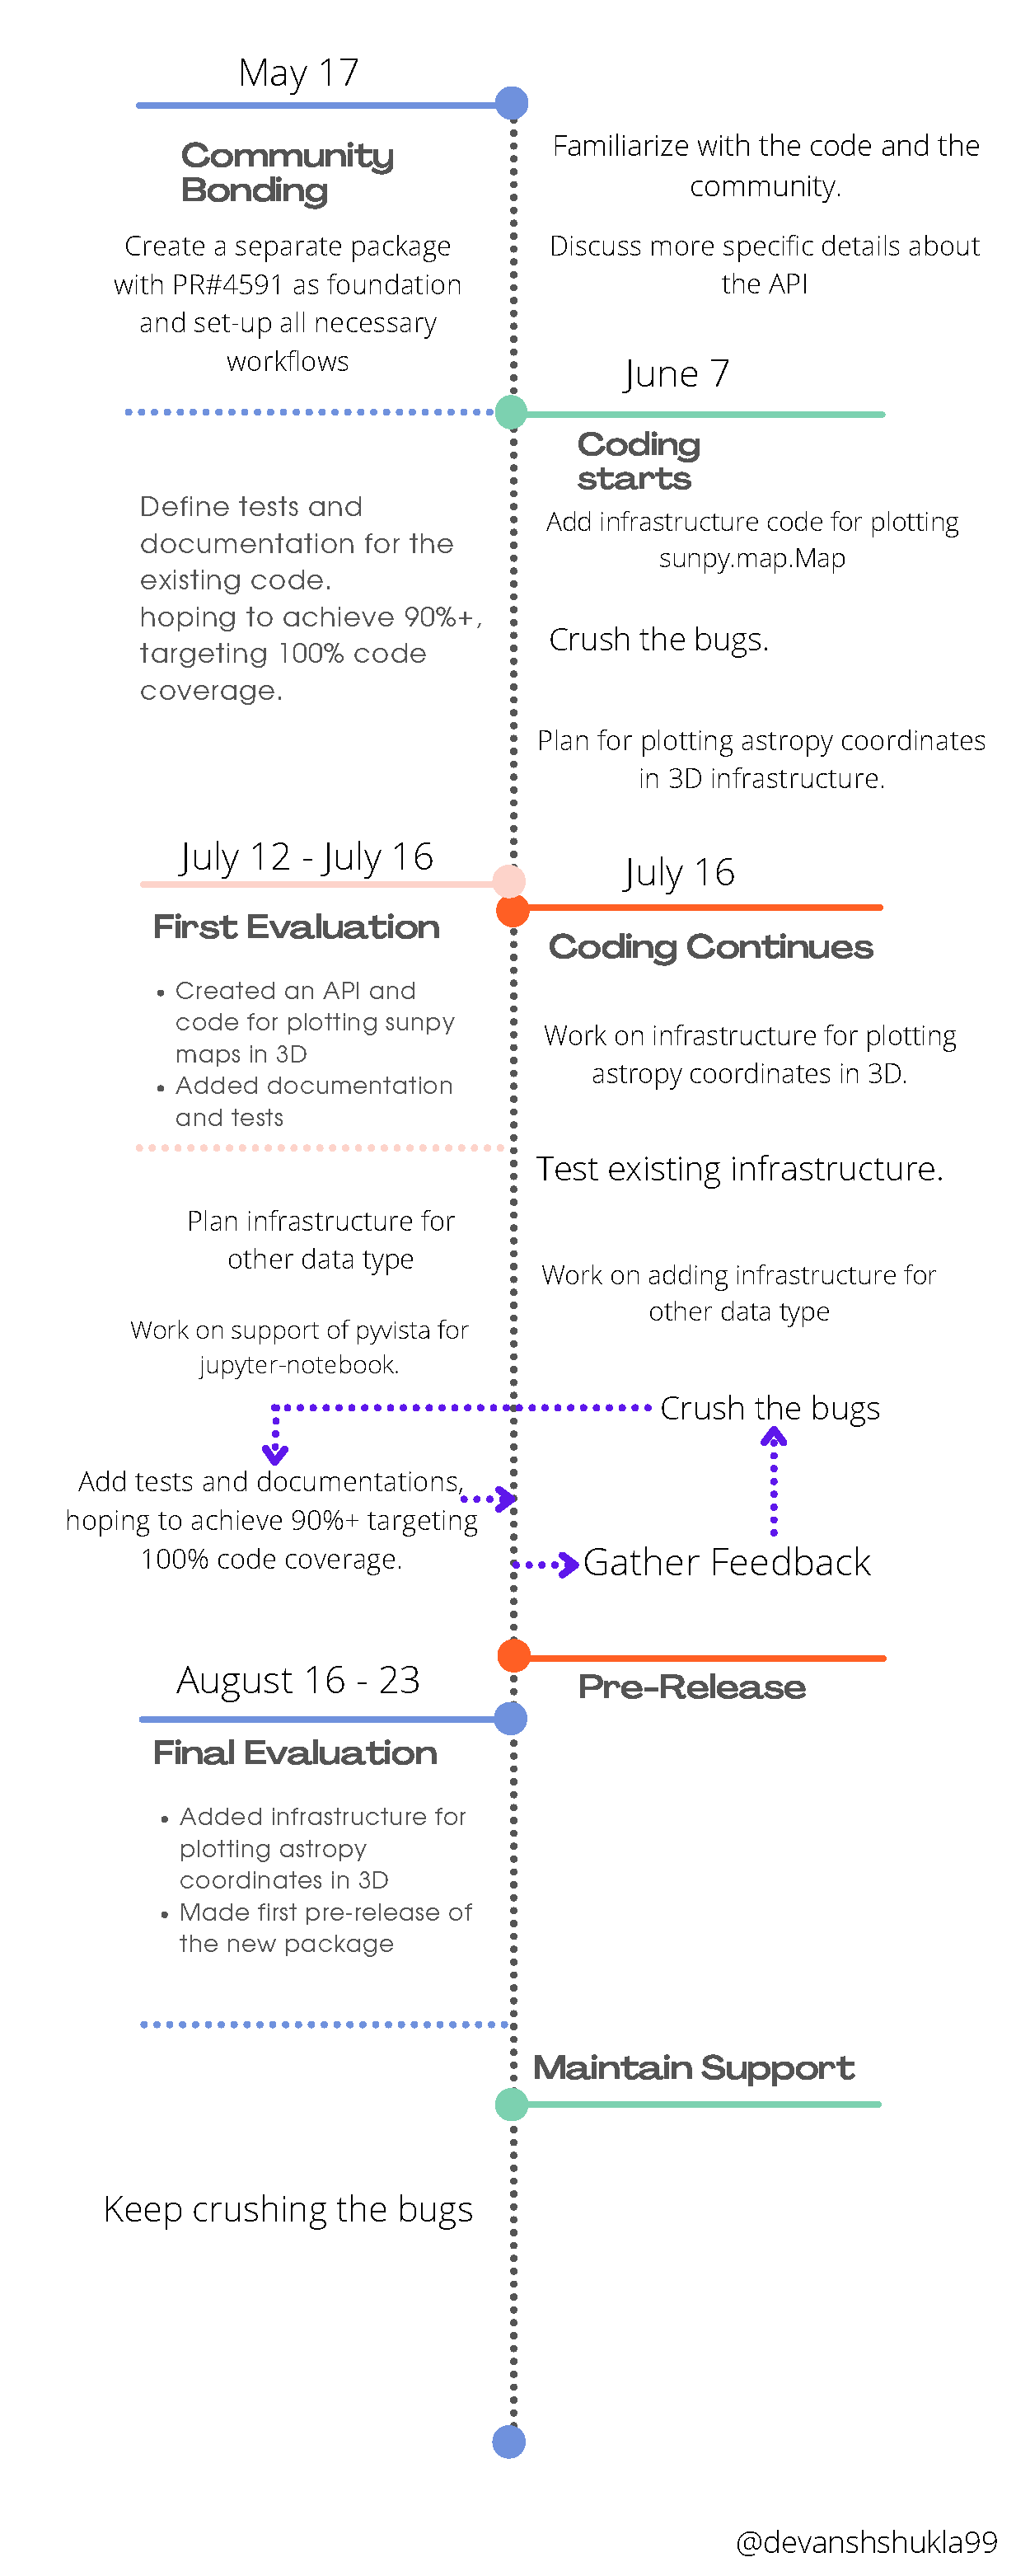
\includepdf[pages={1}, pagecommand=\vspace*{-1cm}\subsubsection{Illustration: Timeline}, scale=0.9]{modules/timeline_devanshshukla99.pdf}
   
    \subsubsection{Verbose Timeline:}
    \vspace*{-0.25cm}
    \begin{itemize}
        \item \textbf{May 17, 2021 - May 24, 2021} \\
            \begin{focus}
                \item Familiarize with the code and the community.
                \item Since I am already familiar with the dev env and test systems used in SunPy(tox, pytest) I'll focus more on the code and how it all is integrated together.
                \item Create a separate package with \pr as foundation and set-up all necessary workflows.
            \end{focus}
        \item \textbf{May 24, 2021 - June 1, 2021} \\
            \begin{focus}
                \item During this time, I'll discuss with my mentors and come with more specific details about the project, like how the public face of the API should behave, etc.
                \item I'll learn and try to solve the challenges I'm already aware-of in the project, see \autoref{subsec:issues_challenges}
                \item Learn more about dependencies like AstroPy, plotly, MPL, PyVista and see how their API is designed.
            \end{focus}
            \item \textbf{May 24, 2021 - June 1, 2021} \\
            \begin{focus}
                \item Plan for the API.
                \item Throughly understand and test the existing code.
                \item Continue learning about the dependencies.
            \end{focus}
        \item \textbf{June 7, 2021 - June 14, 2021} \\
            \begin{focus}
                \item Define tests and documentation for the existing code.
                \item Discuss \& Work on the API.
            \end{focus}
        \item \textbf{June 14, 2021 - June 21, 2021} \\
            \begin{focus}
                \item Add code for plotting sunpy.map.Map
                \item Work on the API.
                \item Crush the bugs along the way.
            \end{focus}
        \item \textbf{June 21, 2021 - June 28, 2021} \\
            \begin{focus}
                \item Add tests and documentation, hoping to achieve 75\%+ code coverage.
                \item Check the Integration with SunPy. -- Waypoint - 1 Check
            \end{focus}
        \item \textbf{June 21, 2021 - June 28, 2021} \\
            \begin{focus}
                \item Crush the bugs.
                \item Add tests and documentation, hoping to achieve 90\%+ targeting 100\% code coverage.
                \item Finalizing the API.
            \end{focus}
        \item \textbf{June 28, 2021 - July 5, 2021} \\
            \begin{focus}
                \item Gather Feedback.
                \item Finalizing the API for the evaluation.
                \item Crush the Bugs.
            \end{focus}
        \item \textbf{July 5, 2021 - July 12, 2021} \\
            \begin{focus}
                \item Finalizing the API for the evaluation.
                \item Plan for plotting astropy coordinates in 3D infrastructure.
                \item Buffer time.
            \end{focus}
        \item \textbf{July 12, 2021 - July 16, 2021} \\
            \begin{focus}
                \item Buffer time, for incorporating required changes as per feedback.
                \item More debugging.
            \end{focus}
        \item \textbf{June 16, 2021 - July 23, 2021} \\
            \begin{focus}
                \item Work on infrastructure for plotting astropy coordinates in 3D.
                \item Discuss on adding infrastructure for other data type.
            \end{focus}
        \item \textbf{July 23, 2021 - July 30, 2021} \\
            \begin{focus}
                \item Test infrastructure for plotting astropy coordinates in 3D.
                \item Plan infrastructure for other data type, SOHO, EUV, RHEISSI, tbd.
                \item Buffer time to crush bugs.
            \end{focus}
        \item \textbf{July 30, 2021 - August 6, 2021} \\
            \begin{focus}
                \item Work on adding infrastructure for other data type, SOHO, EUV etc, tbd.
                \item Add tests and documentations, hoping to achieve 75\%+.
            \end{focus}
        \item \textbf{August 6, 2021 - August 13, 2021} \\
            \begin{focus}
                \item Work on support of pyvista for jupyter-notebook.
                \item Crush the bugs.
                \item Finalize the API.
            \end{focus}
        \item \textbf{August 13, 2021 - August 20, 2021} \\
            \begin{focus}
                \item Add tests and documentations, hoping to achieve 90\%+ targeting 100\% code coverage.
                \item Finalize the API, prepare for the pre-release.
                \item Crush the bugs.
                \item Check Documentation for mistakes/typos/bugs.
            \end{focus}
        \item \textbf{August 13, 2021 - August 16, 2021} \\
            \begin{focus}
                \item Finalize the API, incorporate the feedback from additional review.
                \item Crush the bugs.
                \item Gather feedback.
            \end{focus}
        \item \textbf{August 16, 2021 - August 23, 2021} \\
            \begin{focus}
                \item Pre-Release. 
                \item Crush the Bugs.
            \end{focus}
        \item \textbf{August 23, 2021 - } \\
            \begin{focus}
                \item Maintain support and work on improving the performance and stuff.
                \item Keep crushing the bugs.
            \end{focus}
    \end{itemize}